\documentclass[a4paper,english,12pt]{article}
\usepackage{%
	amsfonts,%
	amsmath,%	
	amssymb,%
	amsthm,%
	algorithm,%
	babel,%
	bbm,%
	etex,%
	%biblatex,%
	caption,%
	centernot,%
	color,%
	dsfont,%
	enumerate,%
	epsfig,%
	epstopdf,%
	geometry,%
	graphicx,%
	hyperref,%
	latexsym,%
	mathtools,%
	multicol,%
	pgf,%
	pgfplots,%
	pgfplotstable,%
	pgfpages,%
	proof,%
	psfrag,%
	subfigure,%	
	tikz,%
	ulem,%
	url%
}	
\usepackage[noend]{algpseudocode}
\usepackage[mathscr]{eucal}
\usepgflibrary{shapes}
\usetikzlibrary{%
  	arrows,%
	backgrounds,%
	chains,%
	decorations.pathmorphing,% /pgf/decoration/random steps | erste Graphik
	decorations.text,%
	matrix,%
  	positioning,% wg. " of "
  	fit,%
	patterns,%
  	petri,%
	plotmarks,%
  	scopes,%
	shadows,%
  	shapes.misc,% wg. rounded rectangle
  	shapes.arrows,%
	shapes.callouts,%
  	shapes%
}

\theoremstyle{plain}
\newtheorem{thm}{Theorem}[section]
\newtheorem{lem}[thm]{Lemma}
\newtheorem{prop}[thm]{Proposition}
\newtheorem{cor}[thm]{Corollary}

\theoremstyle{definition}
\newtheorem{defn}[thm]{Definition}
\newtheorem{conj}[thm]{Conjecture}
\newtheorem{exmp}[thm]{Example}
\newtheorem{assum}[thm]{Assumptions}
\newtheorem{axiom}[thm]{Axiom}

\theoremstyle{remark}
\newtheorem{rem}{Remark}
\newtheorem{note}{Note}
\newtheorem{fact}{Fact}

\newcommand{\norm}[1]{\left\lVert#1\right\rVert}
\newcommand{\indep}{\!\perp\!\!\!\perp}
\DeclarePairedDelimiter\abs{\lvert}{\rvert}%
\newcommand\numberthis{\addtocounter{equation}{1}\tag{\theequation}}
\newcommand{\tr}{\operatorname{tr}}
\newcommand{\R}{\mathbb{R}}
\newcommand{\N}{\mathbb{N}}
\newcommand{\E}{\mathbb{E}}
\newcommand{\Z}{\mathbb{Z}}
\newcommand{\B}{\mathscr{B}}
\newcommand{\C}{\mathcal{C}}
\newcommand{\T}{\mathscr{T}}
\newcommand{\F}{\mathcal{F}}
\newcommand{\G}{\mathcal{G}}
%\newcommand{\ba}{\begin{align*}}
%\newcommand{\ea}{\end{align*}}
\DeclareMathOperator*{\argmax}{arg\,max}
\renewcommand{\qedsymbol}{$\blacksquare$}
\makeatletter
\def\BState{\State\hskip-\ALG@thistlm}
\makeatother

\makeatletter
\def\th@plain{%
  \thm@notefont{}% same as heading font
  \itshape % body font
}
\def\th@definition{%
  \thm@notefont{}% same as heading font
  \normalfont % body font
}
\makeatother
\date{}
\usepackage{amsmath}

\newcommand{\bx}{\mathbf{x}}
\newcommand{\by}{\mathbf{y}}
\newcommand{\bX}{\mathbf{X}}
\newcommand{\bY}{\mathbf{Y}}
\newcommand{\btheta}{\boldsymbol{\theta}}
\newcommand{\bLambda}{\boldsymbol{\Lambda}}


%opening

\title{Lecture 12: Detection of Signals With Random Parameters}
\date{18 Feb 2016}
\author{}

\begin{document}
\maketitle
In the previous lecture the detection of deterministic signals was dealt with. In this lecture, the focus will be on deciding between signals that are known except for a set of unknown random parameters. For this situation the hypothesis testing problem can be conveniently written as,
\begin{equation}
 \label{n1}
      \begin{aligned}
      & H_0 : Y_k=N_k+s_{0k}(\Theta) ,\ \ \ \ k=1,2,3,...n  \\
      \mbox{versus} & \\
      & H_1 : Y_k=N_k+s_{1k}(\Theta) ,\ \ \ \ k=1,2,3,...n
      \end{aligned}
 \end{equation}
 where $\Theta$ is an unknown parameter taking values from a parameter set $\Lambda$. Density of $\Theta$ is $\omega_j$ under the hypothesis $H_j$, $j\in \{0,1\}$. Moreover, $\underline{N}$ is random noise which is independent of the signal and hence independent of $\Theta$.
 The likelihood ratio for \eqref{n1} is given by,
 \begin{equation*}
 L(\underline{y})=\frac{\mathbbm{E}_1 \lbrace p_{\underline{N}}(\underline{y}-\underline{s}_1(\Theta))\rbrace}{\mathbbm{E}_0 \lbrace p_{\underline{N}}(\underline{y}-\underline{s}_0(\Theta))\rbrace}  \ \ \  \forall \underline{y}\in \R^ n
 \end{equation*}
 Here $\mathbbm{E}_j$ denotes the expectation under density $\omega_j$. 
 \begin{equation}
 \label{n3}
 L(\underline{y})=\frac{\int_\Lambda  p_{\underline{N}}(\underline{y}-\underline{s}_1(\theta))\omega_1(\theta)\mu (d\theta)}{\int_\Lambda  p_{\underline{N}}(\underline{y}-\underline{s}_0(\theta))\omega_0(\theta)\mu (d\theta)} 
 \end{equation}
  Without loss of generality, we can assume that $\underline{s_0}\equiv 0$ and $\underline{s_1}\triangleq \underline{s}$. Applying this in \eqref{n3}, we have
\begin{align} 
 L(\underline{y})&=\int_\Lambda \frac{ p_{\underline{N}}(\underline{y}-\underline{s}(\theta))}{p_{\underline{N}}(\underline{y})}\omega(\theta)\mu (d\theta) \\ 
  \label{n5}
 &=\int_\Lambda L_\theta(\underline{y})\omega(\theta)\mu (d\theta)  
\end{align} 
where $L_\theta(\underline{y})$ is likelihood ratio conditioned on $\Theta = \theta$.
\section{ Noncoherent Detection of a Modulated Sinusoidal Carrier}
\par Now let us consider an example for this case, where noncoherent detection of a modulated sinusoidal carrier is done.
\begin{equation*}
      \begin{aligned}
      & H_0 : s_0(\theta)=\underline{0} \\
      & H_1 : s_1(\theta)=\underline{s}(\theta) = (s_k(\theta))_{k=1}^n
      \end{aligned}
\end{equation*}
 where $s_k(\theta)$ is given by,
 \begin{equation*}
     s_k(\theta) = a_k sin[(k-1)\omega_c T_s+\theta]\ \ \ \ k=1,2,3,...n
 \end{equation*}
where $a_1,a_2,...,a_n$ are a known amplitude sequence and $\Theta$ is random phase uniformly distributed in the interval [0,$2\pi$], and where $\omega_c$ and $T_s$ are a known carrier frequency and sampling interval respectively with relationship $n(\omega_cT_s)=m(2\pi)$ for some integer m. Choice of m is in such a way that the number of samples taken per cycle of the sinusoid is an integer greater than 1 (i.e, m divides n). These signals provide a model for a digital signalling scheme in which a "zero" is transmitted by sending nothing and "one" is transmitted by sending a signal modulated by a sinusoidal carrier of frequency $\omega_c$ (oftenly called On-Off Keying). \\
Assuming i.i.d. $\mathcal{N}(0,\sigma^2)$ noise, the likelihood ratio in \eqref{n5} can be rewritten as,
\begin{equation}
 \label{n8}
 L(\underline{y})=\frac{1}{2\pi}\int_{0}^{2\pi} exp\bigg(\frac{1}{\sigma^2}\big(\sum_{k=1}^{n}y_k s_k(\theta)-\frac{1}{2}\sum_{k=1}^{n}s_k^2(\theta)\big)
\bigg)d\theta
\end{equation}
The first term in paranthesis in the exponent in \eqref{n8} can be written as:
\begin{align}
\sum_{k=1}^{n}y_k s_k(\theta) &= \sum_{k=1}^{n} a_k y_k[sin[(k-1)\omega_c T_s] cos\theta+cos[(k-1)\omega_c T_s] sin\theta] \\
 \label{n10}
&= y_c sin\theta +y_s cos\theta
\end{align}
The equation in \eqref{n10} is obtained by using the identity $sin(A+B)=sinAcosB+cosAsinB$. Moreover $y_c$ and $y_s$ are defined as follows:
\begin{equation*}
y_c \triangleq \sum_{k=1}^{n}a_k y_k cos[(k-1)\omega_c T_s]
\end{equation*}
\begin{equation*}
y_s \triangleq \sum_{k=1}^{n}a_k y_k sin[(k-1)\omega_c T_s]
\end{equation*}
Now we consider the second term in paranthesis in the exponent in \eqref{n8}
\begin{align*}
-\frac{1}{2}\sum_{k=1}^{n}s_k^2(\theta) &= -\frac{1}{2}\sum_{k=1}^{n}a_k^2\bigg[\frac{1}{2}-\frac{1}{2}cos[2(k-1)\omega_c T_s+2\theta]\bigg] 
\end{align*}
\begin{align}
 \label{n14}
&=-\frac{1}{4}\sum_{k=1}^{n}a_k^2+\frac{1}{4}\sum_{k=1}^{n}a_k^2 cos[2(k-1)\omega_c T_s+2\theta]
\end{align}
\par The equation in \eqref{n14} above is obtained using the identity $sin^2A= \frac{1}{2}-\frac{1}{2}cos2A$.
For most of the situations in practice, the second term in \eqref{n14} is zero or approximately zero for all values of $\theta$. For example, if the signal sequence $a_1,a_2,...,a_n$ is a constant times the sequence of $\pm1$'s or if $a_1,a_2,...,a_n$ has a raised cosine shape, then the above second term is identically zero. In other cases of interest, the sequence $a_1^2,a_2^2,...,a_n^2$ is slowly varying as compared to twice the carrier frequency. So the above second term amounts to low pass filtering of a high frequency signal, which yields a negligible output. Thus $L(\underline{y})$ becomes
\begin{equation}
 \label{n15}
L(\underline{y})=exp\bigg(-\frac{n\bar{a^2}}{4\sigma^2}\bigg)  \frac{1}{2\pi}\int_{0}^{2\pi}exp\bigg[-\frac{1}{\sigma^2}( y_c sin\theta +y_s cos\theta)\bigg]d\theta
\end{equation}
where
\begin{equation}
 \label{n16}
\bar{a^2}=\frac{1}{n}\sum_{k=1}^{n}a_k^2
\end{equation}
The integral term in \eqref{n15} can be written as
\begin{equation}
 \label{n17}
\frac{1}{2\pi}\int_{0}^{2\pi}exp\bigg[-\frac{1}{\sigma^2}( y_c sin\theta +y_s cos\theta)\bigg]d\theta= I_0\bigg(\frac{r}{\sigma^2}\bigg)
\end{equation}
where $r=\sqrt{y_c^2+y_s^2}$ and $I_0$ is the modified Bessel function of first kind and order zero. We know that $I_0(x)$ is monotonic in $x$. Hence the optimum tests in this case can be given as
\begin{align}
 \label{n18}
\tilde{\delta}_0 (\underline{y}) =  
\begin{cases}
1 &>  \\
\gamma  \ \ \ \  if \ r&= \sigma^2I_0^{-1} (\tau e^{\frac{n\bar{a^2}}{4\sigma^2}}) \\
0 &<
\end{cases}
\end{align}
\begin{figure}[hbtp]
	\centering
	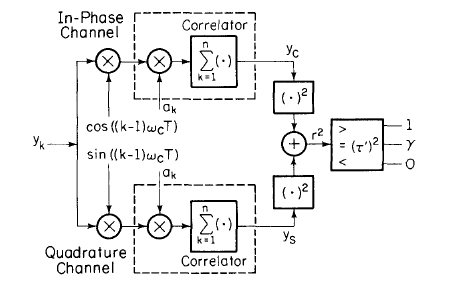
\includegraphics[scale=0.75]{Figures/VP_III_B_10.png}
	\caption{Optimum system for noncoherent detection of a modulated sinusoid in i.i.d. Gaussian noise  \\ \textit{(Source: H. Vincent Poor, An Introduction to Signal Detection and Estimation(Second
			Edition), Figure III.B.10)}}
	\label{fn1}
\end{figure}
The structure of the detector is as shown in the  Figure \ref{fn1}. The observed signal $y_1,y_2,...,y_n$ is split into two channels one being in-phase channel and the other quadrature channel.Each channel correlates the resulting product with the amplitude sequence $a_1,...,a_n$. The channel outputs are then combined to give r, which is compared to a threshold.This structure is also called envelope detector.
\section{Performance Analysis of Optimum System for noncoherent detection}
To analyze the performance of the detector, we need to find  $\mathcal{P}_j(\Gamma_1)$, j $\in \{0,1\}$ which is same as $\mathcal{P}_j(R>\tau)$, where $R=Y_c^2+Y_s^2$ and,
\begin{equation*}
Y_c\triangleq\sum_{k=1}^{n}a_k Y_k\cos[(k-1)\omega_c T_s] \ \ 
\end{equation*}
\begin{equation*}
Y_s\triangleq\sum_{k=1}^{n}a_k Y_k\sin[(k-1)\omega_c T_s]
\end{equation*}
The desired probabilities can be found from the joint probability density function of $Y_c$ and $Y_s$ under two hypothesis. \\
Under Hypothesis zero,
\begin{equation*}
H_0: \underline{Y} \sim \mathcal{N}(0,\sigma^2\underline{I})
\end{equation*}
$Y_c$ and $Y_s$ are jointly Gaussian. We can specify the joint density of ($Y_c,Y_s$) under $H_0$ by finding the means and variances of $Y_c$ and $Y_s$, and the correlation coefficient between $Y_c$ and $Y_s$.\\
Clearly,
$$\mathbbm{E}\big\{Y_c|H_0\big\} = \mathbbm{E}\big\{Y_s|H_0\big\} = 0$$
\begin{equation*}
\begin{aligned}
Var\big[Y_c|H_0\big]
&=\sum_{k=1}^{n}\sum_{l=1}^{n}a_k a_l\mathbbm{E}\big\{N_k,N_l\big\}\cos[(k-1)\omega_c T_s]\cos[(l-1)\omega_c T_s] \\
&= \sum_{k=1}^{n}a_k^2\sigma^2\cos^2[(k-1)\omega_c T_s] \\
&= \sum_{k=1}^{n}\frac{a_k^2\sigma^2}{2} \\
&= \frac{\sigma^2n\bar{a^2}}{2}\\
&= Var\big[Y_s|H_0\big]
\end{aligned}
\end{equation*}
Covariance is given by,
\begin{equation*}
\begin{aligned}
Cov\big(Y_c,Y_s|H_0\big) &=\mathbbm{E}\big\{Y_c,Y_s|H_0\big\}\\
&=\sum_{k=1}^{n}\sum_{l=1}^{n}a_k a_l\mathbbm{E}\big\{N_k,N_l\big\}\cos[(k-1)\omega_c T_s]\sin[(l-1)\omega_c T_s] \\
&=\sum_{k=1}^{n}a_k^2\sigma^2\cos[(k-1)\omega_c T_s]\sin[(k-1)\omega_c T_s] \\
&= 0
\end{aligned}
\end{equation*}
\par Since covariance of $Y_c$ and $Y_s$ is zero, $Y_c$ and $Y_s$ are uncorrelated. This implies $Y_c$ and $Y_s$ 
are independent (For Gaussian random variables uncorrelatedness implies independence).\\
The false alarm probability thus becomes,
\begin{equation*}
\begin{aligned}
\mathcal{P_F}(\tilde{\delta}_{NP}) &=\mathcal{P}_0(\Gamma_1)   
= \mathcal{P}_0(Y_c^2+Y_s^2>(\tau')^2) \\
&=\iint \limits_{(y_c^2+y_s^2>(\tau')^2)}^{} \frac{1}{\pi n\sigma^2\bar{a^2}}  \exp\bigg(\frac{ -(y_c^2+y_s^2)}{n\sigma^2\bar{a^2}}\bigg)dy_c dy_s \\
&=\int \limits_{\psi=0}^{2\pi}\int \limits_{r=\tau'}^{\infty}\frac{r}{\pi n\sigma^2\bar{a^2}}   \exp\bigg(\frac{ -r^2}{n\sigma^2\bar{a^2}}\bigg)dr d\psi  \\
&=\exp\bigg(\frac{-(\tau')^2}{n\sigma^2\bar{a^2}}\bigg)  \\
\end{aligned}
\end{equation*}
\par To find detection probability $\mathcal{P}_1(\Gamma_1)$, we need to find the joint density of ($Y_c,Y_s$) under $H_1$. We know that given $\Theta=\theta$, \underline{Y} has a conditional $\mathcal{N}(\underline{s}(\theta),\sigma^2I)$ distribution under $H_1$. So, given $\Theta=\theta$, $Y_c$ and $Y_s$ are conditionally jointly Gaussian.     
\begin{equation*}
\begin{aligned}
\mathbbm{E}\big\{Y_c|H_1, \Theta=\theta\big\} &= \sum_{k=1}^{n}a_k\mathbbm{E}\big\{Y_k|H_1, \Theta=\theta\big\}\cos[(k-1)\omega_c T_s] \\
&=\sum_{k=1}^{n}a_k^2 \sin[(k-1)\omega_c T_s+\theta]\cos[(k-1)\omega_c T_s] \\
&=\sum_{k=1}^{n}a_k^2 \frac{\sin\theta}{2} \\
&=\frac{n\bar{a^2}}{2}\sin\theta
\end{aligned}
\end{equation*}
Similarly, 
\begin{equation*}
\mathbbm{E}\big\{Y_s|H_1, \Theta=\theta\big\}=
\frac{n\bar{a^2}}{2}\cos\theta
\end{equation*} \\ \\
\par With $\theta$ fixed, the variances and covariance of $Y_c$ and $Y_s$ under $H_1$ is same as their corresponding variances and covariance under $H_0$ since the only change in $\underline{Y}$ is a shift in mean. So,
\begin{equation*}
Var\big[Y_c|H_1, \Theta=\theta\big]=
Var\big[Y_s|H_1, \Theta=\theta\big] \\
=Var\big[Y_c|H_0\big] \\
=\frac{\sigma^2n\bar{a^2}}{2} \\
\end{equation*}
\ \ \ \ \  \ $Cov\big(Y_c,Y_s|H_1, \Theta=\theta\big)=0$ \\
Hence the joint unconditioned pdf of $Y_c$ and $Y_s$ under $H_1$ is obtained by averaging the conditional density over $\theta$:
\begin{equation*}
\begin{aligned}
f_{Y_c,Y_s}\big(y_c,y_s|H_1\big)
&=\frac{1}{2\pi} \int_0^{2\pi}f_{Y_c,Y_s}\big(y_c,y_s|H_1, \Theta=\theta\big) d\theta \\
&=\frac{1} {2\pi} \int_0^{2\pi} \frac{1}{\pi n\sigma^2\bar{a^2}} \exp\bigg(\frac{ -q(y_c,y_s;n\bar{a^2}/2,\theta)}{n\sigma^2\bar{a^2}}\bigg) d\theta
\end{aligned}
\end{equation*}
where \textit{q(a,b;c,$\theta$)}=(a-c$\cos\theta)^2$+(b-c$\sin\theta)^2$ \\
Detection Probability thus becomes,
\begin{equation*}
\begin{aligned}
\mathcal{P_D}(\tilde{\delta}_{0}) 
&=\mathcal{P}_1(\Gamma_1)   
= \mathcal{P}_0(Y_c^2+Y_s^2>(\tau')^2) \\
&= \int\limits_{\psi=0}^{2\pi}\int \limits_{r=\tau'}^{\infty}\bigg(\frac{e^{(-n\bar{a^2}/4\sigma^2)}}{\pi n\sigma^2\bar{a^2}}\bigg) r  \exp\bigg(\frac{ -r^2}{n\sigma^2\bar{a^2}}\bigg) \mathcal{I}_0\bigg(\frac{r}{\sigma^2}\bigg)dr d\psi  \\
&=\int \limits_{x=\tau'}^{\infty}x\exp\bigg(-\frac{(x^2+b^2)}{2}\bigg)\mathcal{I}_0\big(bx\big) dx \\
&=\mathcal{Q}(b,\tau_0) \ \ \ \ \ \ \ 
\begin{cases}
b^2 &=n\bar{a^2}/2\sigma^2\\
\tau_0 &= \tau'/ \sigma^2b\\
x  &=  r/\sigma^2b
\end{cases} \ \ \ \ \ \ \bigg(Marcum's \ \ Q-function\bigg)
\end{aligned}
\end{equation*}
We set the threshold $\tau'$ for $\alpha$-level  Neyman-Pearson detection in this problem  as follows. 
\begin{equation*}
\begin{aligned}
\mathcal{P}_0(\Gamma_1)  =  \mathcal{P_F}(\tilde{\delta}_{NP})  =  \alpha \\
\Rightarrow  \exp\bigg(\frac{ -(\tau')^2}{n\sigma^2\bar{a^2}}\bigg)=\alpha \\
\Rightarrow
\tau'= \sqrt{n\sigma^2\bar{a^2}\log\bigg(\frac{1}{\alpha}\bigg)} 
\end{aligned}
\end{equation*}
which gives Receiver operating characteristics(ROCs) as,
\begin{equation*}
\begin{aligned}
P_D(\tilde{\delta})=\mathcal{Q}\bigg(b,\sqrt{2\log\bigg(\frac{1}{\alpha}\bigg)}\bigg)
\end{aligned}
\end{equation*}
 \par Receiver operating characteristics look very similar to those for the coherent problem (Figure \ref{fn2}). 
\begin{figure}[hbtp]
	\centering
	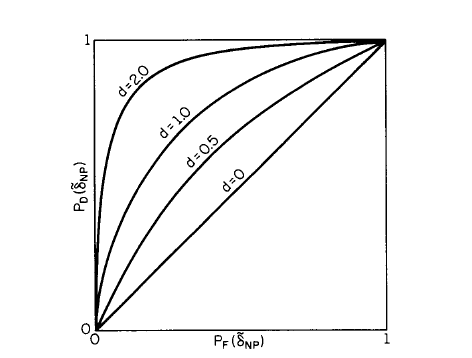
\includegraphics[scale=0.75]{Figures/VP_II_D_4.png}
	\caption{Receiver operating characteristics (R.O.Cs) for Neyman-Pearson non coherent detection with i.i.d. Gaussian noise.  \\ \textit{(Source: H. Vincent Poor, An Introduction to Signal Detection and Estimation(Second
			Edition), Figure II.D.4)}}
	\label{fn2}
\end{figure}
We see that the performance of Neyman-Pearson detection depends only on the parameter b. The average signal energy is given by
\begin{equation}
 \label{n19}
\mathbbm{E}\bigg\{\frac{1}{n}\sum_{k=1}^{n}s_k^2(\Theta) \bigg\}=\frac{1}{n}\frac{1}{2\pi}\int_{0}^{2\pi}\sum_{k=1}^{n}a_k^2sin^2[(k-1)\omega_cT_s+\theta]d\theta = \frac{\bar{a^2}}{2}
\end{equation} 
\par Here $b^2$ has a signal-to-noise ratio interpretation similar to $d^2$ in coherent detection problem. If $\theta$ is known, to detect the same signal coherently, the value of $d^2$ would be
\begin{equation}
 \label{n20}
d^2=\frac{1}{\sigma^2}\sum_{k=1}^{n}s_k^2(\theta)=\frac{1}{\sigma^2}\sum_{k=1}^{n}a_k^2sin^2[(k-1)\omega_c T_s+\theta]=\frac{n\bar{a^2}}{2\sigma^2}=b^2
\end{equation}
\par Thus these signal-to-noise ratios are same. However, the performance for fixed $\alpha$ is different for the two systems. For typical SNR and $\alpha$ values, we have
\begin{equation}
 \label{n21}
\mathcal{Q}\bigg(b,\sqrt{2log\frac{1}{\alpha}}\bigg)  =1-\Phi(\Phi^{-1}(1-\alpha)-d)
\end{equation} 
and the equality holds when $b\approx d+0.4$. This means that we need a slightly higher SNR to get the same performance as that of coherent technique.
\end{document}